\section{Connected Worlds}\label{sec:connected_worlds}


\subsection{Introduction}\label{sec:connected_worlds_intro}
Connected Worlds\footnote{\url{https://nysci.org/home/exhibits/connected-worlds/}} (CW) is a multi-person ecology simulation with the goal of teaching students about complex systems and systems thinking.  It consists of an immersive environment comprising four interconnected biomes and a central flow of water that is fed by a waterfall. Students plant trees which flourish or die, animals arrive or depart, and rain clouds form, move through the sky and deposit rain into the waterfall. All the while, students direct the water stream to different areas in the simulation to provide enough water to sustain plant and animal life. The simulation exhibits large scale feedback loops and presents the opportunity for participants to experience how their actions can have (often unintended) effects that are significantly removed in time and/or space.

Students interact with CW by positioning logs to control the direction of the water that flows in the simulation and by planting trees in the different biomes. Water can be directed to each of the four biomes (Desert, Plains, Jungle and Wetlands) and the distribution of flowing water depends on the placement of the logs. Water on the floor of the simulation (representing a flood plain) is a usable resource as it can then be directed to the biomes. Certain sources of water are under the students' direct control and others are out of their control. Students can actively release water into the system from the water that is stored in the Reservoir or from surplus water that is present in a specific biome. Rainfall events are out of the students' control and these release water into the Waterfall (to replenish the primary source of water) and into the individual biomes. The Mountain Valley can also receive rain and it forms a river source when this happens. Figure~\ref{fig:connected_worlds_graphic} shows a bird's eye snapshot view of the state of logs and water in the simulation in CW. Not seen in this snapshot are the plant and animal counts or levels in the biomes. The volume of water that is stored in each of the biomes is also not shown.

\begin{figure}
\centering
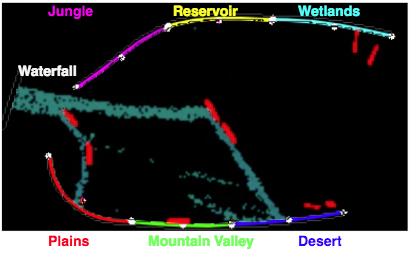
\includegraphics[width=10cm]{connected_worlds_schematic.png}
\caption{Bird's eye view of the CW simulation. Biomes are labeled on the perimeter and logs appear as thick red lines. Water enters via the waterfall and in this image it is mainly flowing from left to right toward the Desert and the Plains.}
\label{fig:connected_worlds_graphic}
\end{figure}




\subsection{Water Cycle}
Every biome in CW shares the common water resource. The amount of water for a given simulation is pre-defined, thus it forms a \textit{limited resource} that students are required to manage carefully. CW simulates a water cycle where water is directed to biomes and used to sustain plants and animals. Evaporation, dependent on the numbers and levels of plants, and rainfall, dependent on the amount of evaporation, brings the water back to the water sources where it once again becomes a usable resource.

\begin{figure}
\centering
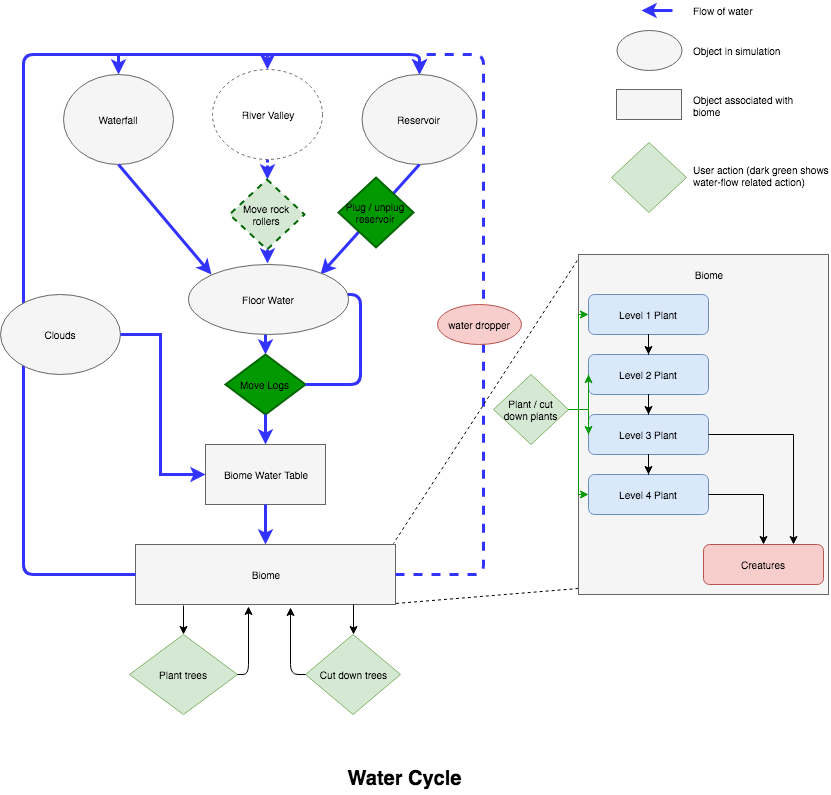
\includegraphics[width=\textwidth]{system_overview_water.png}
\caption{Flow chart showing the water cycles that are present in CW. Blue solid lines represent main water flows, dotted lines represent other possible flows of water that are often not present or are negligible. Green, diamond boxes represent the actions that the students can take that will change the water cycles that are present. Grey circles are regions of the simulation and grey boxes are specifically one of the four biomes.}
\label{fig:system_overview_water}
\end{figure}

Figure \ref{fig:system_overview_water} displays a schematic of the water cycle that is present in CW. Water is available from three sources: the Waterfall, the Mountain Valley and the Reservoir. The Waterfall flows whenever water is available and thus the amount of input water from the Waterfall is out of the students' control. The Mountain Valley is a secondary source of water and it only flows when it rains in this area\footnote{System parameters allow the rain in the Mountain Valley to be turned off, stopping the flow from this area. The rain in the Mountain Valley has been disabled for the experiments presented in this study}. Students choose when to release water from the Reservoir and thus, apart from overflow events, this source of water is directly under their control. Overflow events result when it rains in the Reservoir and the water `spills' out onto the simulation floor when the Reservoir is at full capacity. Students position the logs on the floor of the simulation (see Figure~\ref{fig:connected_worlds_graphic}) to direct some portion of water to some subset of the four biomes. Once a biome has water, the students are able to plant trees. Higher level trees require the presence of lower level trees. The number and level of trees affects the amount of water that the biome requires. Lastly, when water is present in a biome, students can pipe water out of the biome by placing a log at that biome's wall (one of the purple, aqua, red or blue lines in Figure~\ref{fig:connected_worlds_graphic}).



\subsection{Plant-Animal Relations}

Students plant trees and observe the arrival of animals that use the trees to support their habitat. Mimicking a real-world scenario, the fauna for a biome depends on the flora, and the flora are unique for a specific biome. In other words, each biome can support different plants and each type of plant attracts a certain type of animal. Larger and higher level plants require the presence of smaller and lower level plants. Often the animals that are supported by the top level (level 4) plants are the most aesthetically pleasing, and part of the goal for a given simulation might be to attract these animals. Students are thus required to manage their resources to support lower level plants and animals before achieving the top level in a specific biome. The plant and animal relationships are summarized in Figure~\ref{fig:system_overview_plant_animal}.

\begin{figure}
\centering
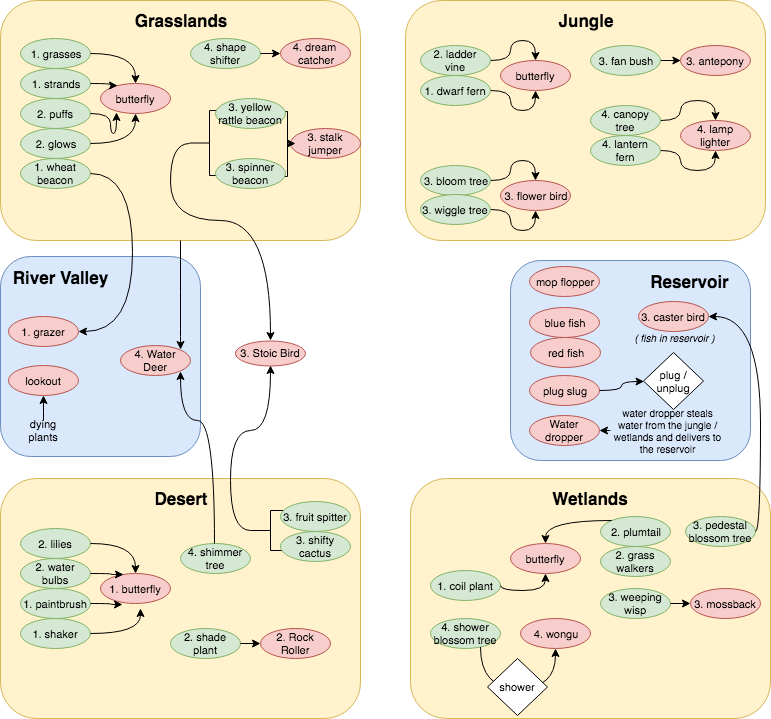
\includegraphics[width=\textwidth]{system_overview_plant_animal.png}
\caption{Map of the relationships between plants, animals and biomes in the CW environment. The biomes are shown in yellow. The blue boxes correspond to areas of the simulation that do support animals but do not have plants that grow there. The fauna-flora specific relations can clearly be seen by the arrows that link the plants (green ovals) and animals (red ovals). The plants and animals are endemic to their biome.}
\label{fig:system_overview_plant_animal}
\end{figure}

\section{Need for Assistive Technology}\label{sec:need_for_assistive_tech}
The nature of the simulation is complex on a variety of dimensions. The simulation involves a large number of students simultaneously executing actions that change the state of the simulated environment.  No one person - including the teacher or interpreter - can possibly follow what happens, even in a relatively short simulation. Each participant may have a different view of what transpired, depending on the actions he or she took and the state changes that resulted. We propose that it is important to develop tools that can support teachers' understanding of the effects of students' interactions in complex exploratory learning environments such as CW. We introduce a technique for decomposing a complex session into shorter periods where the dynamics of the simulation are stable. Our hypothesis is that these smaller periods will individually be more interpretable than the session as a whole and they will eventually form a subset of useful information that a teacher can draw on when leading a review of the session with groups of students.
